\chapter{Equation of State Table Extension}\label{EOStables}

In this study we consider atmosphere growth in the outer parts of protoplanetary disks ($5<a<100$ AU), where temperature and pressure drop to as little as $T \sim 20$ K and $P \sim4\times10^{-6}$ dyn cm$^{-2}$ for our fiducial disk model (see equations \ref{eq:diskb} and \ref{eq:Pd}). We model the nebular gas using the EOS tables of \citet{saumon95}. However, these tables only cover the relatively high temperature and pressure ranges $2.1 < \log_{10} T(\rm{K})<7.06$ and $4.0<\log_{10}P$(dyn cm$^{-2})<19.0$. We thus need to extend the tables to lower $T$ and $P$. We calculate $\delad$ for

\begin{eqnarray}
1.0 & < & \log_{10} T <2.1 \\ 
-5.4& < & \log_{10} P<4.0 
\end{eqnarray} 
using the following method.



%In this section we explain the procedure for extending and interpolating the \cite{saumon95} EOS tables. The EOS takes into account non ideal interactions, and includes physical treatments of dissociation and ionization. However, the \cite{saumon95} EOS tables only cover a relatively high range of temperatures and pressures: $2.10 < \log_{10} T(\rm{K})<7.06$ and $4<\log_{10}P$(dyn cm$^{-2})<19$. We consider cold disks, where the temperature and pressure drop to $\sim 20$ K and $\sim 10^{-4}$ dyn cm$^{-2}$, respectively (see equations (\ref{eq:diskb}) and (\ref{eq:Pd})). It is therefore necessary to extend the \cite{saumon95} EOS tables to lower temperature and pressure values.

%We choose $\log_{10} T (\rm{K})=1$ and $ \log_{10}P$(dyn cm$^{-2})=-4.4$ as our lower boundaries for temperature and pressure, respectively. Our temperature and pressure grid becomes: $1 < \log_{10} T(\rm{K})<7.06$ and $-4.4<\log_{10}P$(dyn cm$^{-2})<19$. The other thermodynamic variables in the tables are calculated as follows.

\section{Hydrogen}

\label{hydrogen}

Following \citet{kittel}, we calculate $\delad$ from the partition function for the internal energy of a system of hydrogen gas molecules (see also \citealt{dangelo13} for EOS calculations that take into account hydrogen isomers).  We begin by writing the partition function $Z$ of a gas molecule of mass $m$ as the product of the partition functions associated with each type of internal energy:

%\begin{equation}
%\label{eq:z}
%Z=Z_t Z_r Z_v Z_e Z_n,
%\end{equation}

\begin{equation}
\label{eq:zagain}
Z=Z_t Z_r Z_v \;\;,
\end{equation} 

\noindent where $Z_t$, $Z_r$, $Z_v$ are associated with translation, rotation, and vibration, respectively.\footnote{We ignore electronic and nuclear excitation as they are only important at temperatures much higher than our regime of interest.}  %For hydrogen, electronic and nuclear excitation are only significant at temperatures higher than our region of interest ($\theta_e \approx 12000$ K and $\theta_n >> \theta_e$, where $\theta_e$ and $\theta_n$ are the characteristic temperatures for electronic and nuclear excitation, respectively). As such, we will only take into account the translation, rotation and vibration of the hydrogen molecule:

%In what follows we present and briefly derive expressions for thermodynamic variables based on quantum mechanics principles. More details on the derivations can be found in \citet{kittel}.

In the classical limit, the molecule's center of mass motion generates

\begin{equation}
\label{eq:Zt}
Z_t=(m k_B T/2 \pi \hbar^2)^{3/2} V,
\end{equation}
where  $T$ and $V$ are the gas temperature and volume, respectively, and $\hbar$ is the reduced Planck constant. The rotational partition function is

\begin{equation}
\label{eq:Zr}
Z_r=\sum_{j=0}^\infty (2 j+1) \exp{\Big[\frac{-j (j+1)\Theta_r}{T}\Big]},
\end{equation}

\noindent where the characteristic temperature for rotational motion $\Theta_r \approx 85$ K  for hydrogen. However, molecular hydrogen occurs in two isomeric forms: parahydrogen with a symmetric (even) rotational wavefunction, and orthohydrogen with an antisymmetric (odd) wavefunction (see Section \ref{deladtable}). %Parahydrogen with an even rotational wave function, while orthohydrogen can only have an antisymmetric (odd) wave function. 
The rotational partition functions for ortho- and parahydrogen are thus
\begin{equation}
\label{eq:Zpara}
Z_{\rm{r,para}}=\sum_{j=0}^\infty \frac{1+(-1)^j}{2} (2 j +1) \exp\Big[-\frac{j(j+1)\Theta_r}{T}\Big]
\end{equation}
and
\begin{equation}
\label{eq:Zortho}
Z_{\rm{r,ortho}}=3\sum_{j=0}^\infty \frac{1-(-1)^j}{2} (2 j +1) \exp\Big[-\frac{j(j+1)\Theta_r}{T}\Big] \;\;.
\end{equation}
The factor of 3 in Equation (\ref{eq:Zortho}) accounts for the three-fold degeneracy of the ortho state.

 In thermal equilibrium, the spin isomers have a combined partition function $Z_{\rm r}=Z_{\rm{r, ortho}}+Z_{\rm{r,para}}$, which can be written

\begin{equation}
\label{eq:Zrspin}
Z_r=\sum_{j=0}^\infty (2-(-1)^j) (2j+1) \exp{\Big[\frac{-j (j+1) \Theta_r}{T}\Big]} \;\;.
\end{equation}
For a fixed 3:1 ortho-to-para ratio, the combined partition function is $Z_{\rm r}=Z_{\rm r,para}^{1/4} Z_{\rm r, ortho}^{3/4}$. In our range of temperatures of interest, we find that $Z_r$ converges after about 25 terms in the series, for both the equilibrium and 3:1 cases.

Note that $Z_{\rm r, ortho} \rightarrow 0$ and $Z_{\rm r,para} \rightarrow 1$ as $T \rightarrow 0$. This is inconsistent with a fixed 3:1 ortho-to-para ratio, since $Z_{\rm r, ortho} \rightarrow 0$ implies that there is no orthohydrogen in the system. \citet{boley07} and \citet{dangelo13} ensure that this requirement is not violated by using a normalized orthohydrogen partition function,  $Z'_{\rm r, ortho}=Z_{\rm r, ortho} \exp(2 \theta_{\rm r}/T)$, which reduces the energy of the lowest rotational state for orthohydrogen from $2k_{\rm B}\theta_{\rm r}$ per molecule to zero. This decreases the total internal energy of the system by a constant factor, but does not change $c_{\rm v}$, $\delad$, or the relative internal energies of static atmospheric profiles, and therefore does not affect atmospheric evolution.

Finally, the partition function for vibrational motion is given by:

\begin{equation}
\label{eq:Zv}
Z_v=[1-\exp{(\theta_v/T)}]^{-1},
\end{equation}

\noindent where the characteristic temperature for vibrational motion is $\theta_v  \approx 6140$ K for hydrogen. 

For a system of $N$ particles of mass $m$, the partition function of the ensemble is $Z_{\rm N}=(1/N!)Z^N$. Given $Z_{\rm N}$ as a function of $(V, T)$, the internal energy per mass, entropy per mass and specific heat capacity can be written as

%\begin{equation}
%\label{eq:U}
%U_N=k T^2 \Big(\frac{\partial \log{Z}}{\partial T}\Big)_{V, N}
%\end{equation}
%
%\begin{equation}
%\label{eq:S}
%S_N=k \log{Z} + \frac{U_N}{T}
%\end{equation}
%
%The energy, and entropy per mass and specific heat capacity will subsequently be:

\begin{equation}
\label{eq:u}
u=\mathcal{R}T^2 \Big(\frac{\partial \ln{Z}}{\partial T}\Big)_{V}
\end{equation}
%{\bf CHANGED BIG U TO LITTLE u IN EQUATIONS BELOW: CONFIRM}
\begin{equation}
\label{eq:s}
S=\mathcal{R} \ln{Z} + \frac{u}{T}-\frac{\mathcal{R}}{N} \ln N!
\end{equation}
\begin{equation}
\label{eq:cv}
c_{\rm V}=\Big(\frac{\partial u}{\partial T}\Big)_{V}.
\end{equation}
Note that, following the convention of \citet{saumon95}, we use $S$ to denote entropy per mass ($[S]=$erg K$^{-1}$ g$^{-1}$).  Since $Z=Z_t Z_r Z_v$, we may write $u=u_t+u_r+u_v$ and $S=S_t+S_r+S_v$, where variables subscripted $t$, $r$, and $v$ are the quantities corresponding to the individual translation, rotation and vibration partition functions, respectively. We include the term $\mathcal{R}/N \ln N!$ from Equation (\ref{eq:s}) in $S_{\rm t}$.

%\textbf{Using the translational partition function, internal energy and entropy expressions for an ensemble of $N$ identical particles of mass $m$, i.e. $Z_N=(1/N!) Z_t^N$, $U_N=k_B T^2 (\partial \ln{Z_N}/\partial T)_{V, N}$, and $S_N=k_B \ln{Z_N} + U_N/T$, Stirling's approximation $\ln N! \approx N \ln N-N,$ and the ideal gas law $P=\rho \mathcal{R} T$, the {\bf resulting} entropy per mass due to translational motion can be expressed as:}

 In the temperature regime for which the rotational states of $\rm{H}_2$ are selectively occupied, the total number of particles in the system is constant and we may use the ideal gas law, $P=\rho \mathcal{R} T$. With Equations (\ref{eq:u}), (\ref{eq:s}), and Stirling's approximation, $\ln N! \approx N \ln N-N$, the resulting entropy per mass due to translational motion is

\begin{equation}
\label{eq:st}
S_{\rm t}=\mathcal{R} \Big[ \frac{5}{2} \ln{T} - \ln{P} + \ln \Big( \frac{(2 \pi)^{3/2} \mathcal{R}^{5/2} m^4}{h^3}\Big) +\frac{5}{2} \Big]
\end{equation}
Equation (\ref{eq:st}) is known as the Sackur-Tetrode formula. % \textbf{and is only applicable to an ideal gas REALLY? WE'RE USING IT FOR THE TRANSLATIONAL COMPONENT IN A NON-IDEAL GAS}. 
%\textbf{We can use the ideal gas law to derive Equation (\ref{eq:st}) for the $\rm{H}_2$ molecule because the total number of particles in the system, and hence the mean molecular weight and specific gas constant $\mathcal{R}$, do not change with temperature in the regime where the rotational states are selectively occupied.} 

The internal energy per mass due to translational motion is given by:

\begin{equation}
\label{eq:ut}
u_t=\frac{3}{2} \mathcal{R} T
\end{equation}

Putting all of the above together, we can now evaluate the thermodynamic quantities needed to extend the \cite{saumon95} EOS tables to low temperatures and pressures.

\begin{enumerate}

\item{\textbf{Density.}} In the low temperature, low pressure regime, $\rho$ is related to $T$ and $P$ by the ideal gas law. %hydrogen is molecular and behaves like an ideal gas. As such, the density in this region follows the ideal gas law $P=\rho \mathcal{R} T$.
\item{\textbf{Internal energy per mass.}} $u=u_t+u_r+u_v$, where $u_t$ is given by Equation (\ref{eq:ut}), and $u_r$ and $u_v$ are determined using Equations (\ref{eq:Zrspin}), (\ref{eq:Zv}) and (\ref{eq:u}) above.
\item{\textbf{Entropy per unit mass}}. Similarly, $S=S_t+S_r+S_v$, where $S_t$ is given by Equation (\ref{eq:st}), and $S_r$ and $S_v$ can be determined from Equation (\ref{eq:s}) and the calculated expressions for $u_r$ and $u_v$, respectively.
\item{\textbf{Entropy logarithmic derivatives}}. The logarithmic derivatives $S_T$ and $S_P$ are given by:

\begin{equation}
\label{eq:sT}
S_T=\frac{\partial \ln{S}}{\partial \ln{T}} \Big |_P
\end{equation}
and
\begin{equation}
\label{eq:sP}
S_P=\frac{\partial \ln{S}}{\partial \ln{P}} \Big |_T
\end{equation}
We calculate $S_T$ and $S_P$ through finite differencing. 

\item{\textbf{Adiabatic gradient $\delad$}}. The adiabatic gradient is defined as:

\begin{equation}
\label{eq:deladSP}
\delad=\frac{\partial \ln{T}}{\partial \ln{P}} \Big |_S = -\frac{S_P}{S_T}
\end{equation}

\begin{figure}[H]
\centering
%\includegraphics[scale=.8]{../../figs/ModelAtmospheres/RadSelfGravRealEOS/PaperFigs/delad_S_H.pdf}
\includegraphics[scale=.7]{figures/delad_S_H.pdf}
\caption{Contour plot of the hydrogen adiabatic gradient $\delad$ as a function of gas temperature and pressure. The upper right rectangle encloses the region described by the original \citet{saumon95} EOS tables, while the rest of the plot is our extension to lower temperatures and pressures for an equilibrium mixture of ortho- and parahydrogen. The black curves represent constant entropy adiabats with labels $\log_{10}(S)$, where $S$ [erg K$^{-1}$ g$^{-1}$] is the absolute entropy per unit mass.  At high temperatures, hydrogen dissociates and ionizes, while at low temperatures the rotational states of the hydrogen molecule are only partially excited and it no longer behaves like an ideal diatomic gas. Regions in which the EOS is invalid or has not been computed are masked in white (see text).}
\label{fig:deladH}
\end{figure}

We evaluate $\delad$ from the tabulated values for $S_T$ and $S_P$ determined above. Figure \ref{fig:deladH} shows a contour plot of $\delad$ as a function of temperature and pressure for the extended EOS table for hydrogen, assuming thermal equilibrium between the spin isomers. For the 3:1 ortho-to-para ratio, $\delad$ decreases continuously with $T$ for $T \lesssim 200$ K, in contrast with the equilibrium case, in which $\delad$ sharply decreases, then increases as $T$ goes down. Our extension is only valid for $T \lesssim 2000$ K, since it does not take into account hydrogen dissociation. We choose $T=1500$ K as a conservative temperature cutoff. While we account for vibrational motion for completeness, its contribution is negligible in the temperature regime of interest. \citet{saumon95} do not compute the EOS at very high pressures, since hydrogen is solid or may form a Coulomb lattice in this regime, and thus their EOS treatment is no longer valid. While the boundaries of the region in which the free-energy EOS treatment fails can be determined from fundamental thermodynamic constraints, such calculations are not the object of this work. Instead, we choose as boundary a constant entropy curve ($\log(S)=8.4$) above the region in which the \citet{saumon95} model fails. The expressions derived above are sufficient to give good results for the colored regions of the extended map, which fully cover the temperature and pressures ranges required by our models.

 %Our extension smoothly matches the original tables for $8.80<\log{S}$(K g$^{-1})<9.07$ (\textbf{numbers are wrong, change once you have the final figure version}).

\end{enumerate}


\section{Helium}

We extend the helium EOS tables based on a similar procedure. Since helium is primarily neutral and atomic at low temperatures and pressures, we treat it as an ideal monoatomic gas and  only take into account the translational component of the partition function (\ref{eq:Zt}). Figure \ref{fig:deladHe} shows $\delad$ as a function of temperature and pressure for the extended EOS table. %The original and extended table join smoothly for entropy curves between $8.29<\log{S}$(K g$^{-1})<8.77$ in this case (\textbf{numbers are wrong, change once you have the final figure version}).

\begin{figure}[H]
\centering
%\includegraphics[scale=.8]{../../figs/ModelAtmospheres/RadSelfGravRealEOS/PaperFigs/delad_S_He.pdf}
\includegraphics[scale=.7]{figures/delad_S_He.pdf}
\caption{Same as Figure \ref{fig:deladH} but for pure helium. Helium ionizes at $T \gtrsim 10,000$ K, but behaves as an ideal monatomic gas otherwise. We choose $T=7,000$ K as a conservative temperature cutoff above which our  extension is no longer valid (masked in white). The EOS has not been computed in the lower-right region of the plot (see text).}
\label{fig:deladHe}
\end{figure}

\vspace{0.2in}

Lastly, we combine Figures \ref{fig:deladH} and \ref{fig:deladHe} to obtain EOS tables for a hydrogen-helium mixture using the procedure described in \citet{saumon95}.  Figure \ref{fig:deladmap} displays results for helium mass fraction $Y=0.3$.

%Using equation (\ref{eq:upartition}) we therefore recover the standard result $U_{\rm r}=\mathcal{R} T$ (refs). Furthermore, we know that the internal energy and entropy per unit mass associated with translation are given by $U_{\rm t}=\frac{3}{2} \mathcal{R}$ and $C_{\rm{v,t}}=\frac{3}{2}\mathcal{R}$, respectively, and so we are able to calculate the total internal energy and specific heat of a diatomic molecule as a function of temperature. An example of the variation of heat capacity with temperature is shown in \citet{kittel}, chapter 3. 

%The partition function associated with rotation is generally written as:
%
%\begin{equation}
%\label{eq:Zr}
%Z_{\rm r}=\sum_0^\infty (2 j +1) \exp\Big[-\frac{j(j+1)\Theta_r}{T}\Big],
%\end{equation}
%with $j$ the angular momentum quantum number \citep{kittel}. Various thermodynamic quantities can be derived from the partition function. For example, the internal energy per unit mass can be written as:
%
%\begin{equation}
%\label{eq:upartition}
%u_{\rm r}=\mathcal{R}T^2 \frac{\partial \log Z}{\partial T}
%\end{equation}
%
%The specific heat at constant volume then easily follows as
%
%\begin{equation}
%\label{eq:cvpartition}
%c_{\rm{v,r}}=\Big(\frac{\partial u}{\partial T}\Big)_V
%\end{equation} 

